\documentclass[tikz,border=5mm]{standalone}
\begin{document}
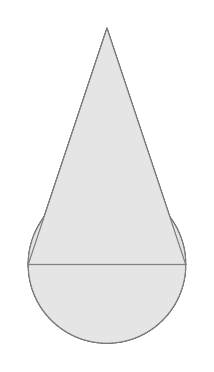
\begin{tikzpicture}
    % 绘制圆锥体
    \draw (0,0) circle (1cm);
    \draw (0,3) -- (1,0);
    \draw (0,3) -- (-1,0);
    
    % 填充圆锥体
    \filldraw[fill=gray!20!white, draw=gray] (0,0) circle (1cm);
    \filldraw[fill=gray!20!white, draw=gray] (0,3) -- (1,0) -- (-1,0) -- cycle;
\end{tikzpicture}
\end{document}